%%%%%%%%%%%%%%%%%%%%%%%%%%%%%%%%%
\subsection{Tracing Methods for Vectorization}

One of the successful earlier methods in image vectorization is called tracing, and at the time was synonymous with image vectorization. The general intuition behind this is that a raster image can be thought of as a collection of adjacent image patches, and we can vectorize an image by detecting edges of shapes.

\begin{figure}
    \centering
    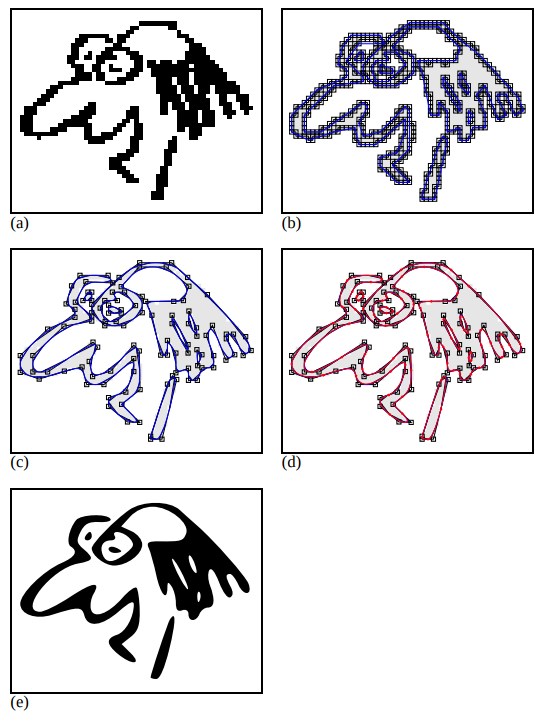
\includegraphics[width=\textwidth]{Figures/potrace.png}
    \caption{An illustration of the Potrace \cite{selinger2003potrace} vectorization process}
    \label{fig:potrace}
\end{figure}

A noteworthy implementation of image tracing is the Potrace algorithm \cite{selinger2003potrace}. As the name suggests, Potrace first attempts to convert a raster image into a series of polygonal paths via edge detection and straight-line detection, and then attempts to simplify (optimize) polygons by reducing path cardinalities and introducing Bezier curves. It employs many useful heuristics to improve image quality, such as removing speckles smaller than a given ``turd size'', detecting and smoothing corners, redundancy coding in the target format, scaling and rotating a small set of parameterized curves, and data quantization. An illustration of the stages of the Potrace algorithm is shown in \cref{fig:potrace}. The implementation of Potrace is open-source, and the program is highly configurable via command-line options.

This interpretation of vectorization is useful for simple raster images that are indeed a collection of adjacent shapes, such as map data, floor charts, typography, or charts. For such images, the Potrace algorithm is both reliable and efficient. While we do not use Potrace in our implementation, we may borrow some of its features related to curve optimization when simplifying the shapes (this is future work).

One of the drawbacks of tracing is that we can only trace edges on a binary thresholded image; if there aren't clearly defined edges, or if there are image gradients (as is often the case), it doesn't represent an image as well. Tracing can be applied to color images by thresholding the image by color or brightness level, and producing vector images for each thresholded layer, but this may seem choppy and low-quality. Tracing also does not recognize non-contiguous shapes (e.g., simple shapes that intersect other shapes), which can allow for more aggressive optimization and better object recognition. Machine learning approaches are better at recognizing this (citation).

%%%%%%%%%%%%%%%%%%%%%%%%%%%%%%%%%
\subsection{Machine Learning Approaches to Vectorization}

\begin{figure}[H]
    \centering
    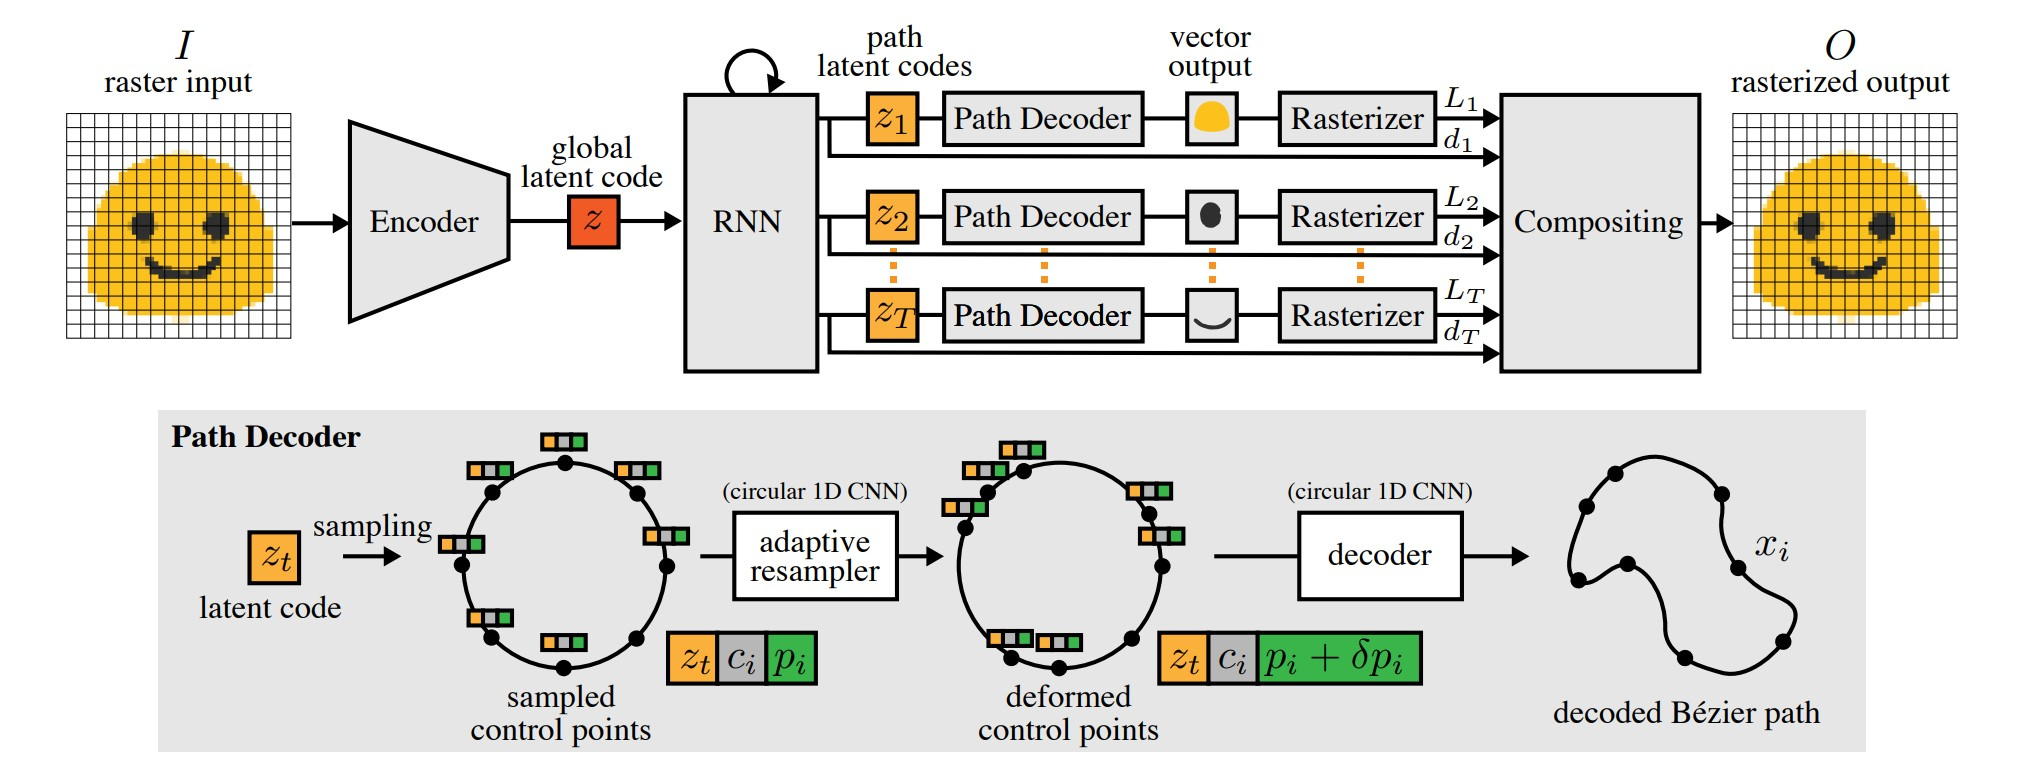
\includegraphics[width=\linewidth]{Figures/im2vec_architecture.jpg}
    \caption{Architecture overview for Im2Vec from \cite{reddy2021im2vec}}
\end{figure}

Im2Vec is an end-to-end deep neural network introduced by \customcite{reddy2021im2vec}. The model takes a raster image as input and outputs an SVG image. The raster image is first passed through an encoder. The encoded representation is then passed through a Recurrent Neural Network (RNN), specifically a bidirectional Long Short-Term Memory network (LSTM), to produce an arbitrary number outputs. Each output is passed through a path decoder, which produces a Bézier path. 

The path decoder uses continuous deformation of the unit circle to ensure each path is closed. The authors sample points on the unit circle and concatenate the output of the RNN to each of the sampled points. The authors next use 1D convolutions, equivalent to convolution around the perimeter of the circle, to determine how to deform the unit circle.

This model is trained by appending a differentiable rasterizer to the output. The rasterizer converts the vector output back to raster format and the resulting image can be compared to the original image to compute a loss. Since the rasterizer is differentiable, that loss can be backpropagated through the model. 

We explored using this model as part of our approach, but after looking through the codebase, we discovered that this would likely not work for our purposes. It appears that the authors hard-coded the number of shapes in the input raster image, along with the colors that each shape should be. We are looking to apply our model to various types of architectures, which will likely not be as well-defined as the emojis used in their experiments.

%%%%%%%%%%%%%%%%%%%%%%%%%%%%%%%%%
\subsection{Sampling Methods for Vectorization}

Sampling methods tackle the vectorization problem by stochastically approximating regions of the vector image. This allows us to achieve a reasonable performance and accuracy. Sampling methods may approximate edges less accurately than edge tracing, but they can overcome some of tracing's limitations, namely being limited to binary thresholding. Like tracing methods, it extends fairly well to more complicated images, while machine learning methods currently appear to be more limited to simple images.

%%%%%%%%%%%%%%%%% Move this citation to the appropriate place
An example procedure for image vectorization through sampling is shown in Zhao et al.'s work \customcite{zhao2013image}. The sampling method for vectorization is composed of 3 steps. The image is first convoluted with a Sobel differential operator to generate an ``importance matrix''. This represents the discontinuities or gradients in the original matrix; larger gradients may indicate regions with more detail. We then apply blue-noise sampling to the image using the importance matrix to determine sampling density around each pixel, with a larger gradient causing a higher sampling density. The sampled points are then triangulated, and the line segments of the triangles form the vector representation of the image. 

%%%%%%%%%%%%%%%%%%%%%%%%%%%%%%%%%
\subsection{Vector Image Optimization}

Several methods for optimizing a polygonal path (i.e., a closed polyline) into a smaller polyline, and by expressing curved sequences of edges as a single Bezier curve, are explored in the Potrace algorithm \cite{selinger2003potrace}. However, this only deals with simplifying curves, while maintaining the overall topology. The sampling method generates a triangulated mesh rather than a sequence of closed paths; in this method, the optimization scheme may look different and may change the overall topology. For example, we do not have any polylines to curve-optimize unless some edges are removed to form non-triangular polygonal patches; it is then a matter of which edges can be removed while retaining fidelity to the original image.

\customcite{hoppe1999new} describes an approach to reduce triangular meshes by merging two adjacent vertices in an arbitrary $n$-dimensional triangular mesh. This technique also results in a triangular mesh, and thus may be useful for 3-D modeling. The method attempts to optimize volume preservation using a quadric error metric and color attribute discontinuities across triangle bounds, illustrated in \cref{fig:edge_collapse}. 

We can be more aggressive than Hoppe's method and not preserve triangular regions, since we are working in a two-dimensional space. We can use their idea of respecting color discontinuities to remove edges, and then perform Potrace's curve optimizations on the resulting polygonal areas.

\begin{figure}
    \centering
    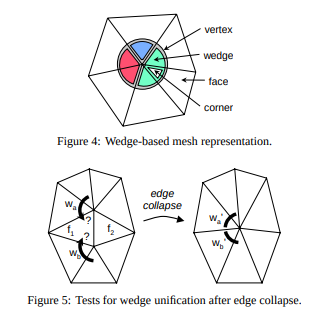
\includegraphics[width=3in]{Figures/edge_collapse.png}
    \caption{Collapsing an edge in \cite{hoppe1999new}, taking into consideration color discontinuities}
    \label{fig:edge_collapse}
\end{figure}
